% !TeX root = ../../main.tex

\subsection{2-DOF Arm Multi-Agent Distributed Experiment}

Since the distributed setup achieves higher performance, we will be moving to a more higher and complex distributed algorithms which provide high-performance throughput and can scale to support multi-agent environments and simulate in a larger scale for achieving faster training and performance in the least amount of time providing high-performance computing power.

\subsubsection{Aim of the experiment}

This experiment is designed to be performed on large multi-agents scale in a distributed setup using APE-X DDPG Algorithm for continuous spaces. Using a single GPU learner and many CPU workers for experience collection. Experience collection can scale to hundreds of CPU workers due to the distributed prioritization of experience prior to storage in replay buffers.

We want to investigate how the agent will perform in the experiment, the time taken to run the experiment, the average episode reward the agent will get and whether the agent will be able to solve the environment in constrained stopping conditions.

\subsubsection{Setup and configurations}

In this experiment, the Distributed Prioritized Experience Replay (Ape-X) algorithm is selected to train the agents in the experiments. Since this experiment is Scalable Multi-Agent, the experiment was performed with multiple numbers of agents and environment per each agent to test the Scalability and efficiency and determine the best setup for the experiment.

The default configuration for  Ape-X  algorithm can be found in the appendix Section~\ref{apex_default}.

In the table below~\ref{tab:gym_reacher_apex_3rd_exp}, the setup and configuration used for the experiment are listed:
\begin{table}[!htb]
	\centering
	\begin{tabular}{|c|l|l|c|l|l|}
		\hline
		\multicolumn{6}{|c|}{\textit{\textbf{Gym Reacher Ape-X 3rd Experiment: Multi-Agent Distributed Experiment}}}                                                        \\ \hline
		\multicolumn{3}{|c|}{\textbf{env}}                                            & \multicolumn{3}{c|}{RoboschoolReacher-v1}                                            \\ \hline
		\multicolumn{3}{|c|}{\textbf{env\_type}}                                      & \multicolumn{3}{c|}{OpenAI Environment}                                              \\ \hline
		\multicolumn{3}{|c|}{\textbf{run: Algorithms}}                                & \multicolumn{3}{c|}{\cellcolor[HTML]{C0C0C0}\textbf{APEX\_DDPG}}                     \\ \hline
		\multicolumn{3}{|c|}{}                                                        & \multicolumn{3}{c|}{\cellcolor[HTML]{E1F7E1}episode\_reward\_mean = 21}              \\ \cline{4-6} 
		\multicolumn{3}{|c|}{\multirow{-2}{*}{\textbf{stop condition}}}               & \multicolumn{3}{c|}{\cellcolor[HTML]{E1F7E1}time-steps\_total = 10000000: 10M Steps} \\ \hline
		\multicolumn{3}{|c|}{\textbf{use\_huber}}                                     & \multicolumn{3}{c|}{True}                                                            \\ \hline
		\multicolumn{3}{|c|}{\textbf{clip\_rewards}}                                  & \multicolumn{3}{c|}{False}                                                           \\ \hline
		\multicolumn{3}{|c|}{\textbf{n\_step}}                                        & \multicolumn{3}{c|}{3}                                                               \\ \hline
		\multicolumn{3}{|c|}{\textbf{exploration\_ou\_noise\_scale}}                  & \multicolumn{3}{c|}{1.0}                                                             \\ \hline
		\multicolumn{3}{|c|}{\textbf{target\_network\_update\_freq}}                  & \multicolumn{3}{c|}{50000}                                                           \\ \hline
		\multicolumn{3}{|c|}{\textbf{tau}}                                            & \multicolumn{3}{c|}{1.0}                                                             \\ \hline
		\multicolumn{3}{|c|}{\textbf{evaluation\_interval}}                           & \multicolumn{3}{c|}{5}                                                               \\ \hline
		\multicolumn{3}{|c|}{\textbf{evaluation\_num\_episodes}}                      & \multicolumn{3}{c|}{MeanStdFilter}                                                   \\ \hline
		\multicolumn{3}{|c|}{\cellcolor[HTML]{C0C0C0}\textbf{num\_gpus}}              & \multicolumn{3}{c|}{\cellcolor[HTML]{C0C0C0}1}                                       \\ \hline
		\multicolumn{3}{|c|}{\cellcolor[HTML]{C0C0C0}\textbf{num\_workers}}           & \multicolumn{3}{c|}{\cellcolor[HTML]{C0C0C0}11}                                      \\ \hline
		\multicolumn{3}{|c|}{\cellcolor[HTML]{C0C0C0}\textbf{num\_envs\_per\_worker}} & \multicolumn{3}{c|}{\cellcolor[HTML]{C0C0C0}grid\_search: [32, 16]}                  \\ \hline
	\end{tabular}
	\caption{Gym Reacher Ape-X 3rd Experiment: Multi-Agent Distributed Experiment}
	\label{tab:gym_reacher_apex_3rd_exp}
\end{table}

As shown in the configuration table~\ref{tab:gym_reacher_apex_3rd_exp} above, we setup the number of environments to be for the first time \textbf{32 per each worker} leading the experiment to have \textbf{384 parallel environment} running in the experiment. The second run of the experiment have \textbf{16 environment per worker}, in this way the experiment have \textbf{192 environment} running in the experiment. The number of the environment can be much bigger that this in there are more powerful computing provided.


\subsubsection{Experiment Results}

The experiment is performed until an average reward of 21 achieved or for a maximum of 10000000 (10M) steps if no improvement is observable. For evaluating the model performance, we compare the average reward between both experiments. In total, we measure the following metrics averaging over each episode:
\begin{itemize}
	\item The Maximum reward the agent can achieve
	\item The Average reward the agent can achieve
	\item The Total Time Steps obtained by the agent
	\item The Total Time taken to perform the experiment
\end{itemize}

Starting from the maximum reward the agent has obtained, the agent could quickly learn and surpass both distributed and non-distributed PPO algorithm after only 2M time-steps. Achieve (+40.4) the maximum reward in the environment. In the following figure~\ref{fig:3rd_exp_max_eps_reward}, the performance of all the agents for the maximum reward in the environment is shown below:
\begin{figure}[H] %[!htb]
	\centering
	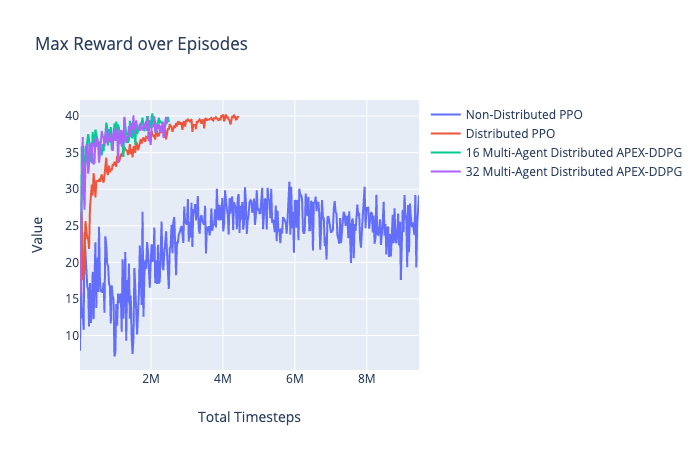
\includegraphics[width=1.2\linewidth]{figures/exps/3rd_exp/max_eps_reward.png}
	\caption{Maximum Reward over Episodes for the 3rd distributed Ape-X DDPG experiment on 2-DOF robotic arm. The maximum reward achieved is +40.4 reward.}
	\label{fig:3rd_exp_max_eps_reward}
\end{figure}

Comparing the performance of the three agents for the average reward. The observation are the distributed apex-ddpg version exceed (+10) average reward after only 100,000 time-steps. Followed by performance improvement over time-steps as the agent reach 21 reward after 2M time-steps, leading the agent to solve the environment and achieve the specified 21 average reward before completing 3M time-steps. Hence, the agent performance is better than the two previous agents and could solve the environment effectively before reaching 3M time-steps. The following figure~\ref{fig:3rd_exp_avg_eps_reward}, illustrate the performance of each agent for obtaining the average rewards.
\begin{figure}[H] %[!htb]
	\centering
	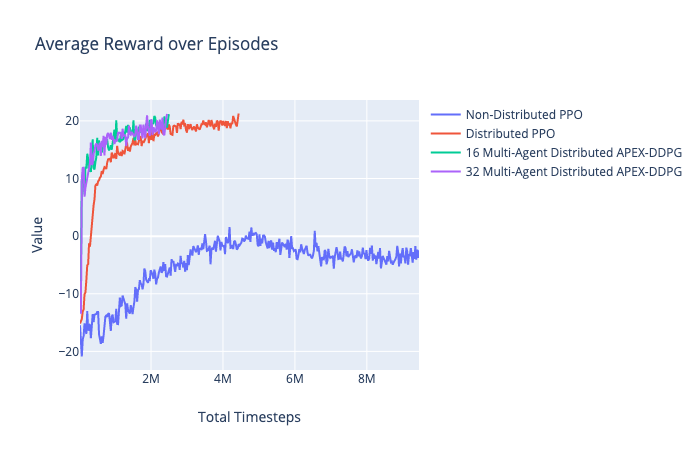
\includegraphics[width=1.2\linewidth]{figures/exps/3rd_exp/avg_eps_reward.png}
	\caption{Average Reward over Episodes for the 3rd distributed Ape-X DDPG experiment on 2-DOF robotic arm. The agent solved the task and get +21.3 reward.}
	\label{fig:3rd_exp_avg_eps_reward}
\end{figure}

The experiment's total taken time is the best factor in this experiment as the algorithm with the huge number of parallel environment was able to finish the task under only (1 Hour) of training. Exceeding the time for both the experiments and utilizing the use of GPU and parallel environment to achieve the goal quickly. Hence, using powerful high-throughput algorithms leads to much faster training time. The following figure~\ref{fig:3rd_exp_total_training_time} show the time taken for each experiment per hour.
\begin{figure}[H] %[!htb]
	\centering
	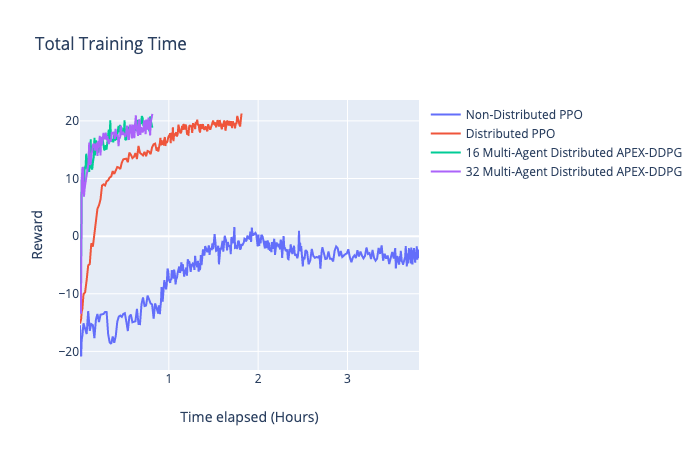
\includegraphics[width=1.2\linewidth]{figures/exps/3rd_exp/total_training_time.png}
	\caption{Total Training Time for the 3rd distributed Ape-X DDPG experiment on 2-DOF robotic arm. Compared with the previous experiments, this agent solved the task faster(\~approximately less than 1 Hours).}
	\label{fig:3rd_exp_total_training_time}
\end{figure}


\subsubsection{Conclusion}

In this experiment, we perform a training and evaluation for the robotic arm using distributed APEX-DDPG algorithm to train our agent. As shown in the results, we conclude that using high-throughput powerful algorithm in a distributed setup leads to have the best outcome for both completing a task and reducing the total time of the experiment.

Summary for the results:
\begin{itemize}
	\item The agent solved the required task.
	\item The agent only required 2.2M time-steps to complete the task.
	\item The average the agent gets 21.5 reward over the whole episodes (figure~\ref{fig:3rd_exp_avg_eps_reward}).
	\item The maximum the agent could get exceed 40.3 reward over the whole episodes (figure~\ref{fig:3rd_exp_max_eps_reward}).
	\item The performance of the agent better than the previous agents.
	\item The total time elapsed did not exceed 1 hours (~47 minutes) (figure~\ref{fig:3rd_exp_total_training_time}).
\end{itemize}